\begin{minipage}{0.63\textwidth}
    \parskip=1em
    \section*{セキュリティモジュール:ピザ}
    
    \uline{概要}:8つの三角形があります。いくつかの三角形が順番通り光っています。

    \uline{解除方法}:すべての正しい三角形を押してください。回答入力欄は最初に三角形を押してから数えて{、}いつも約3\~6秒間有効になります。
\end{minipage}%
\hfill%
\begin{minipage}{0.33\textwidth}
    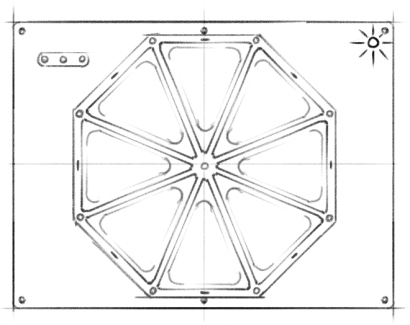
\includegraphics[width=\textwidth]{images/11.png}
    \vspace*{\fill}
\end{minipage}

\uline{押す三角形}:
\begin{itemize}
    \item[$\bullet$] 爆弾のカバーが4つのネジで取り付けられていた場合は{、}点灯した三角形のみを押します。{*}
    \item[$\bullet$] 爆弾のカバーが6つのネジで取り付けられていた場合は{、}点灯しなかった三角形のみを押してください。{*}
\end{itemize}
*以下の例外を参照してください。

\uline{例外}:
\begin{itemize}
    \item[$\bullet$] タイマーのバッテリーに二酸化マンガンリチウム電池が使用されている場合(付録Iを参照){、}北の三角形を押さないでください。
    \item[$\bullet$] 反対側になっているバッテリーホルダーが存在する場合(付録Iを参照){、}南の三角形を押さないでください。
    \item[$\bullet$] タイマーのシリアル番号に少なくとも1つの偶数が含まれている場合は{、}東の三角形を押さないでください。
    \item[$\bullet$] タイマーの通し番号が偶数のみの場合は{、}西の三角を押さないでください。
\end{itemize}

「まだ生きている爆発物処理班」の為のヒント:
\begin{itemize}
    \item[$\bullet$] ゼロも偶数です。
    \item[$\bullet$] 三角形を押して{、}組み合わせが承認または拒否されるまで待ちます。これは3\~6秒以内に行われます。
    \item[$\bullet$] 上記の指示に従ったら押す三角形がなくなった場合は{、}ランダムな三角形を2回押してください。
\end{itemize}
